\documentclass[10pt,a4paper,landscape]{article}

% Packages
\usepackage[utf8]{inputenc}
\usepackage[margin=0.1in]{geometry}
\usepackage{multicol}
\usepackage{amsmath}
\usepackage{amssymb}
\usepackage{enumitem}
\usepackage{titlesec}
\usepackage{xcolor}
\usepackage{graphicx}
\usepackage{multirow}
\usepackage{tikz}
\usepackage{pgfplots}
\pgfplotsset{compat=1.18}
\usepackage{parskip}

% Page setup
\setlength{\parindent}{0pt}
\setlength{\parskip}{0pt}
\setlength{\columnseprule}{0.2pt}
\setlength{\columnsep}{10pt}

% Section formatting
\titleformat{\section}
  {\normalfont\fontsize{5}{6}\bfseries}{\thesection}{1em}{}
\titlespacing*{\subsection}{0pt}{2pt}{0pt}

\titleformat{\subsection}
  {\normalfont\fontsize{5}{6}\bfseries}{\thesubsection}{1em}{}
\titlespacing*{\subsection}{0pt}{2pt}{0pt}

% List formatting
\setlist[itemize]{leftmargin=*, noitemsep, topsep=0pt, parsep=0pt, itemsep=0pt}
\setlist[enumerate]{leftmargin=*, noitemsep, topsep=0pt, parsep=0pt, itemsep=0pt}

% Reduce font size globally
\renewcommand{\normalsize}{\fontsize{5}{6}\selectfont}
\renewcommand{\small}{\fontsize{4}{5}\selectfont}
\renewcommand{\footnotesize}{\fontsize{3}{4}\selectfont}

% Custom chapter header
\newcommand{\chapterheader}[1]{
  \noindent\colorbox{black}{\parbox{\dimexpr\linewidth-2\fboxsep\relax}{%
    \color{white}\bfseries\normalsize #1}}%
  \par\vspace{1pt}
}

% Document settings
\pagestyle{empty}

\begin{document}
\normalsize

\begin{multicols*}{3}


\chapterheader{Chapter 1: Fundamental Concepts in ML}

\begin{itemize}
    \item Classifications vs Regressions
    \item Training vs Testing
    \item Overfitting vs Underfitting (Bias-Variance Tradeoff)
    \item Regardless of which model you use, the most important thing is how it performs with the testing data.
    \item Independent vs Dependent variables. Independent variables are also called features.
    \item Discrete vs continuous data
\end{itemize}


\chapterheader{Chapter 2: Cross Validation}

\begin{itemize}
    \item Problem: how do we pick the best points for training and for testing?
    \item Solution: use cross validation, use all data points for both purposes in an iterative way.
    \item Reusing the same data for training and testing is called data leakage.
    \item Because each iteration uses a different combination of data for training and testing, each fold will give a different fitted model and testing data, resulting in different prediction errors. We can average these errors to get a general sense of the model performance.
    \item Single train/test split is noisy. Cross-validation makes model performance score more reliable.
    \item Leave-One-Out Cross Validation (LOOCV): uses one data point for testing, the rest of the data for training. LOOCV is preferred when the dataset is very small.
    \item Hyperparameter selection: We can compare models/settings fairly using the same CV protocol, pick the best by average score, instead of a single noisy split.
\end{itemize}


\chapterheader{Chapter 3: Fundamental Concepts in Statistics}

\begin{itemize}
    \item Statistics provides a set of tools to quantify the variation that we find in everything and help us make predictions and quantify how confident we should be in those predictions
    \item Histogram: can be used to make classifications using the algorithm called Naive Bayes. Sometimes we have to try a bunch of different bin widths to get a clear picture, bin width too wide or too narrow don't give much info
    \item Probability Distribution: when we don't have much data, and we want to make precise probability estimation, we can use probability distributions. We can use the area under the probability distribution curve to calculate the probability of measuring a value in a range, even when we don't have enough data and there is no data points that fell in the target range
    \item Discrete vs Continuous Probability Distributions
    \item Histograms are discrete distributions itself, but we require a lot of data for reliable estimation (we have blank spaces in histograms if data is not enough)
    \item Binomial distribution equation:
    \[
    p(x \mid n, p) = \left( \frac{n!}{x!\,(n-x)!} \right) p^{x}(1-p)^{\,n-x}
    \]
    \item Binomial distribution is used to calculate the probabilities in any situations that has binary outcomes
    \item Poisson distribution:
    \[
    p(x \mid \lambda) = \frac{e^{-\lambda} \lambda^x}{x!}
    \]
    \item Poisson distribution is used, for example, to calculate the probability of reading exactly 8 pages of a book in the next hour, given that the average speed is 10 pages per hour. $x = 8$ and $\lambda = 10$
    \item Now continuous distributions. One example is the Normal distribution:
    \[
    f(x \mid \mu, \sigma) = \frac{1}{\sqrt{2\pi\sigma^2}} \exp\left(-\frac{(x-\mu)^2}{2\sigma^2}\right) \text{ (probability density function)}
    \]
    \item Knowing the standard deviation is helpful because normal curves are drawn such that 95\% of the measurements fall between $+/-$ 2 standard deviations around the mean
    \item The output from the equation of the normal distribution is a likelihood, NOT a probability
    \item The probability is the area under the curve of pdf. $f(x)$ gives the likelihood. $\int_a^b f(x)\,dx$ gives the probability. The probability for a specific measurement is always 0 (area of zero width is zero). Another way to understand that is, in continuous distributions, the probability for a specific value with infinite precision, is zero
    \item Exponential distributions are commonly used when we are interested in how much time passes between events
    \item Uniform distributions are commonly used to generate random numbers that are equally likely to occur.
    \item Now how can statistics quantify the quality of a model - Sum of the Squared Residuals
    \item Residual = Observed - Predicted
    \item Sum of raw residual values cancel out, so we use the sum of squared residuals to compare. Squaring, instead of taking the absolute value, makes the equation easy to take derivative, which will be handy in gradient descent
    \[
    \text{SSR} = \sum_{i=1}^{n} (\text{Observed}_i - \text{Predicted}_i)^2
    \]
    \item Problem with SSR: it depends on the amount of testing data points. More data has more residuals
    \item Solution: Mean Squared Error, $\text{MSE} = \frac{\text{SSR}}{n}$, where $n$ is the number of observations
    \item Problem with MSE: it depends on the scale of the y-axis. In other words, we cannot compare MSEs where one is 2 millimeters and the other 2 meter
    \item Solution: R-squared value $(R^2)$, it gives the percentage of how much the predictions improved by using the model, instead of just the mean value
    \[
    R^2 = \frac{\text{SSR}(\text{mean}) - \text{SSR}(\text{model})}{\text{SSR}(\text{mean})} \text{ or } R^2 = 1 - \frac{\text{SSR}(\text{model})}{\text{SSR}(\text{mean})}
    \]
    \item In other words, R-squared value puts the error into perspective to the error obtained from the naive average prediction (mean)
    \item R-squared of 0.7 means 70\% reduction in the size of the residuals between the naive mean and the fitted model
    \item Small amount of random data can have a high R-squared value, any time we see a trend in a small dataset, it is difficult to have confidence that a high R-squared value is not due to random chance
    \item Prof. Sandro Lera's class smart-to-stupid ratio: $R^2 = \frac{\text{SSR}(\text{mean})}{\text{SSR}(\text{model})}$, how much better is the fitted model compared to the naive mean
    \item R-squared value can be negative.
    \item Problem: we need to quantify how confident we should be in the results of our analysis. Solution: p-values.
    \item P-values are numbers between 0 and 1 that quantify how confident we should be that A is different from B (as in the example of testing drug types)
    \item Calculated using Fisher’s Exact Test (?)
    \item In practice, the common used threshold is 0.05. Meaning if we conduct the same experiment multiple times, only 5% of those experiments would result in the wrong decision. Other common thresholds are 0.01 and 0.001.
    \item In the example of determining two drugs are the same or not is called hypothesis testing. The null hypothesis is that the drugs are the same, and the p-value helps us decide if we should reject the null hypothesis.
    \item P-value doesn’t imply the effect size (how different is drug A and drug B) is large or small.
\end{itemize}


\chapterheader{Chapter 4: Linear Regressions}
\begin{itemize}
    \item Linear Regression can be fitted using Analytical Solutions as well as using Gradient Descent (Iterative).
    \item Linear Model refers broadly to any method with a linear-in-features decision function, including logistic regression, linear SVMs and ridge/lasso.
\end{itemize}


\chapterheader{Chapter 5: Gradient Descent}
\begin{itemize}
    \item Problem: a major part of machine learning is optimizing a models fit to the data, and an Analytical solution is not always possible
    \item When there's no analytical solution, use Gradient Descent. Gradient Descent is an iterative solution that incrementally steps toward an optimal solution
    \item Take Linear regression for example, we want to know the intercept and the slope that minimize the SSR
    \item Loss Function (or Cost Function) refer to anything we want to optimize when we fit a model to data. For example, we might want to optimize the SSR or MSE
    \item By using the chain rule, we will have a the derivative of the loss function with respect to the parameters (Partial Derivatives)
    \item Each iteration:
    \begin{enumerate}
        \item Evaluate the derivative at the current value for the parameters
        \item Take a step from the current value of parameters, to the negative direction of the gradient, to get close to the optimal parameter (hence minimal loss). Learning rate prevents us from taking steps that are too big and skipping past the lowest point in the curve
        \item Calculate the new parameter values
    \end{enumerate}
    \item Stop when step size is close to 0, or maximum iterations reached
    \item Stochastic Gradient Descent: reduce the amount of computation required to optimize parameters, by randomly selecting ONE data point per step. Regardless of how large your dataset is, only one term is computed per derivative for each iteration
    \item Mini-Batch Stochastic Gradient Descent: instead of one data point, use a batch/subset of data points
    \item Will Gradient Descent always find the best parameter values?
    \begin{itemize}
        \item No, it doesn't always find the global minimum, sometimes it's possible that we are stuck at the local minimum, and because it's not possible to graph the loss function (because of multiple parameters), we might not even know we are in one
    \end{itemize}
    \item What can we do about it?
    \begin{enumerate}
        \item Try using different initialization of parameters that we want to optimize, this might avoid local minimum
        \item Fiddle around with the step size, making it larger may help avoid getting stuck in a local minimum
        \item Use Stochastic Gradient Descent, extra randomness helps avoid getting trapped in a local minimum
    \end{enumerate}
    \item How to choose the batch size of a mini-batch SGD?
    \begin{itemize}
        \item It depends on the computer hardware because the main reason we use SGD is to reduce computation. SGD is memory bound
    \end{itemize}
\end{itemize}


\chapterheader{Chapter 6: Logistic Regression}

\begin{itemize}
    \item Logistic Regression is used for classification
    \item Like Linear Regression, Logistic Regression has metrics similar to the R-squared value to give us a sense of how accurate our predictions will be and it also calculates p-values
    \item The y-axis on a Logistic Regression graph represents the probability and goes from 0 to 1. Usually the threshold for classification is 0.5
    \item Probability vs Likelihood:
\end{itemize}

\begin{center}
\includegraphics[width=0.6\linewidth]{imgs/likelyhood.png}
\end{center}

\begin{itemize}
    \item When fitting the data for Logistic Regression, we want to maximize likelihood rather than minimize sum of squared residuals
    \item We calculate the likelihood for the entire line by multiplying the individual likelihood together. In practice, we usually find the optimal squiggle using gradient descent
    \item To avoid underflow (multiplying a lot of small numbers together which gives a result very close to zero, and computer cannot store), we take log for calculating combined likelihood
    \item Limitation: Logistic regression assumes that we can fit an s-shaped squiggle to the data. If that's not a valid assumption we need to use other models (Decision Tree or SVM or NN), or some other method that can handle more complicated relationships among the data
\end{itemize}


\chapterheader{Chapter 7: Naive Bayes}
\begin{itemize}
    \item The problem: we want to seperate the \textit{Normal} messages from \textit{Spam} messages.
    \item Naive Bayes classifier is one of the simplest but surprisingly effective ML models.
    \item Overview: given the message that begins with ``Dear Friend", and we want to classify it as either \textit{Normal} or \textit{Spam}.
    We will need two different equations, one for \textit{Normal} and one for \textit{Spam}.
    \[
    p(N) \times p(\text{Dear} | N) \times p(\text{Friend} | N)
    \]
    \[
    p(S) \times p(\text{Dear} | S) \times p(\text{Friend} | S)
    \]
    $p(N)$, $p(S)$ are \textbf{Prior Probabilities}. In a nut shell, prior probabilities are just guesses that we make without looking at the contents of a message.
    Whichever equation gives us the larger score, tells us the final classifiction.
    \item The most commonly used version of Naive Bayes is called \textbf{Multinomial Naive Bayes}.
    \begin{enumerate}
        \item Given labeled training data: 8 messages are \textit{Normal}, 4 messages are \textit{Spam}.
        \item Calculate the probabilities of seeing each word given that they came from \textit{Normal} messages, and \textit{Spam} messages.
        \item Calculate the Prior Probabilities $p(N) = \frac{\text{Num Normal}}{Num Total}$ and $p(S) = \frac{\text{Num Spam}}{Num Total}$, derived from the training data.
        \item Finally, we classify ``Dear Friend'' to be \textit{Spam} or \textit{Normal}, based on the final score.
    \end{enumerate}
    \item The reason it is \textbf{naive}, is that the model treats all of the words independently, ignoring word ordering and phrasing. ``Dear Friend'' and ``Friend Dear'' get the same score.
    \item To deal with missing data, Naive Bayes adds something called a \textbf{pseudocount} to each word, which is just an extra value added to each word, so that the probability of an unseen word is never 0.
    \item When we have continuous data, we should use \textbf{Gaussian Naive Bayes}.
    \begin{enumerate}
        \item Given labeled training data, we can calculate the means and standard deviations of each features to draw Normal curves.
        \item Calculate the Prior probabilities similarly.
        \item Calculate the score of each class, by multiplying the prior probabilities, by the likelihood (the y-axis coordinates) of each feature.
        \item Finally, make the classification based on the scores.
    \end{enumerate}
    \item To deal with very small likelihoods, which will cause the computer to \textit{underflow}, we calculate the sum of log-likelihoods, when aggregating for the score.
    \item Q\&A:
    \begin{itemize}
        \item If my continuous data are not Gaussian, can I still use Gaussian Naive Bayes? \newline
        Yes, we can use any statistical distribution in combination with Naive Bayes. For example, we can use \textbf{Exponential Distribution} and the model is called \textbf{Exponential Naive Bayes}.
        \item What if some of my data/features are discrete and some of my data/features are continuous? Can I still use Naive Bayes? \newline
        Yes, we can combine the histogram approach and the distribution approach.
        \item How is Naive Bayes related to Bayes' Theorem? \newline
        \textbf{Bayes' Theorem}:
        \[
        P(A \mid B) = \frac{P(B \mid A) \times P(A)}{P(B)}
        \]
        where $P(A \mid B)$ is the \textbf{posterior probability} (probability of A given B), $P(B \mid A)$ is the \textbf{likelihood} (probability of observing B given A), $P(A)$ is the \textbf{prior probability} (initial probability of A), and $P(B)$ is the \textbf{marginal probability} (total probability of observing B).
        \end{itemize}
\end{itemize}

\chapterheader{Chapter 8: Assessing Model Performance}
\subsection*{Confusion Matrix}
    \begin{center}
    \renewcommand{\arraystretch}{1.4}
    \begin{tabular}{cc|c|c|}
        \cline{3-4}
        & & \multicolumn{2}{c|}{\textbf{Predicted}} \\
        \cline{3-4}
        & & Positive & Negative \\
        \hline
        \multicolumn{1}{|c|}{\multirow{2}{*}{\textbf{Actual}}}
        & Positive & TP & FN \\
        \cline{2-4}
        \multicolumn{1}{|c|}{}
        & Negative & FP & TN \\
        \hline
    \end{tabular}
    \end{center}

\begin{itemize}
    \item $\text{Recall = Sensitivit = True Positive Rate} = \frac{TP}{TP + FN}$ \quad (of all actual positives, how many did we catch?)
    \item $\text{Precision} = \frac{TP}{TP + FP}$ \quad (of all predicted positives, how many are correct?)
    \item $\text{Specificity} = \frac{TN}{TN + FP}$ \quad (of all actual negatives, how many did we identify?)
    \item $\text{False Positive Rate} = \frac{FP}{FP + TN} = 1 - \text{Specificity}$ \quad (of all actual negatives, how many did we misclassify?)
\end{itemize}
    
\subsection*{ROC Curve}
\begin{itemize}
    \item ROC stands for \textbf{Receiver Operating Characteristic}, and the name comes from the graphs drawn during World War II that summarized how well radar operators correctly identified airplanes in radar signals.
    \item AUC stands for \textbf{Area Under the Curve}, which is used for comparing models. The model with larger AUC is genrally better.
    \item Problem: when data are imbalanced, let's say we have more negative class data points in our data. ROC graph is hard to interpret because the False Positive Rate barely budges above 0 before we have 100\% True Positive Rate.
    \item Solution: Precision Recall graph.
\end{itemize}
\noindent
\begin{minipage}[t]{0.48\linewidth}
\centering
\textbf{ROC Curve}\\[2pt]
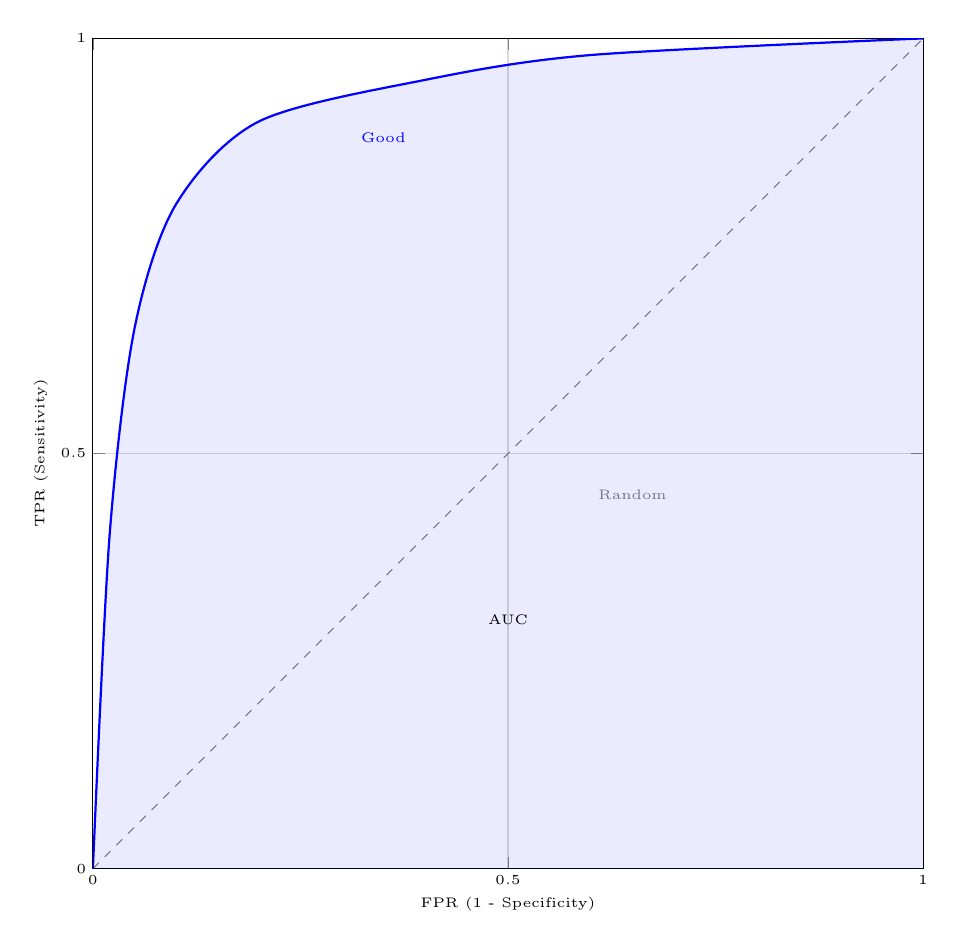
\begin{tikzpicture}
\begin{axis}[
    width=\linewidth,
    height=\linewidth,
    xlabel={FPR (1 - Specificity)},
    ylabel={TPR (Sensitivity)},
    xmin=0, xmax=1,
    ymin=0, ymax=1,
    xtick={0,0.5,1.0},
    ytick={0,0.5,1.0},
    grid=major,
    grid style={gray!30},
    tick label style={font=\footnotesize},
    label style={font=\footnotesize},
]
\addplot[dashed, gray] coordinates {(0,0) (1,1)};
\addplot[thick, blue, smooth] coordinates {
    (0,0) (0.02,0.4) (0.05,0.65) (0.1,0.8)
    (0.2,0.9) (0.4,0.95) (0.6,0.98) (1,1)
};
\node[font=\footnotesize, gray] at (axis cs:0.65,0.45) {Random};
\node[font=\footnotesize, blue] at (axis cs:0.35,0.88) {Good};
\addplot[fill=blue, fill opacity=0.08, draw=none, smooth] coordinates {
    (0,0) (0.02,0.4) (0.05,0.65) (0.1,0.8)
    (0.2,0.9) (0.4,0.95) (0.6,0.98) (1,1)
} -- (axis cs:1,0) -- cycle;
\node[font=\footnotesize] at (axis cs:0.5,0.3) {AUC};
\end{axis}
\end{tikzpicture}
\end{minipage}%
\hfill
\begin{minipage}[t]{0.48\linewidth}
\centering
\textbf{Precision-Recall Curve}\\[2pt]
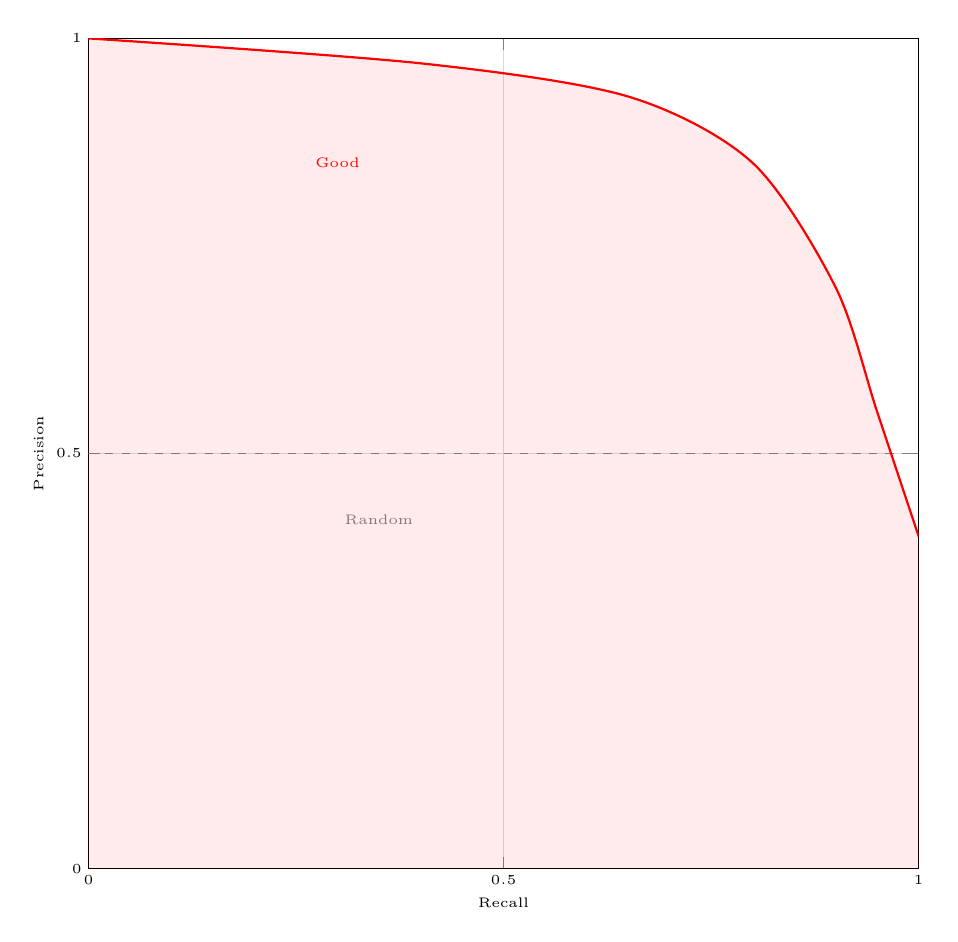
\begin{tikzpicture}
\begin{axis}[
    width=\linewidth,
    height=\linewidth,
    xlabel={Recall},
    ylabel={Precision},
    xmin=0, xmax=1,
    ymin=0, ymax=1,
    xtick={0,0.5,1.0},
    ytick={0,0.5,1.0},
    grid=major,
    grid style={gray!30},
    tick label style={font=\footnotesize},
    label style={font=\footnotesize},
]
\addplot[dashed, gray] coordinates {(0,0.5) (1,0.5)};
\addplot[thick, red, smooth] coordinates {
    (0,1) (0.4,0.97) (0.65,0.93) (0.8,0.85)
    (0.9,0.7) (0.95,0.55) (1,0.4)
};
\node[font=\footnotesize, gray] at (axis cs:0.35,0.42) {Random};
\node[font=\footnotesize, red] at (axis cs:0.3,0.85) {Good};
\addplot[fill=red, fill opacity=0.08, draw=none, smooth] coordinates {
    (0,1) (0.4,0.97) (0.65,0.93) (0.8,0.85)
    (0.9,0.7) (0.95,0.55) (1,0.4)
} -- (axis cs:1,0) -- (axis cs:0,0) -- cycle;
\end{axis}
\end{tikzpicture}
\end{minipage}


\chapterheader{Chapter 9: Preventing Overfitting with Regularization}
\begin{itemize}
    \item \textbf{The Problem}: the fancier and more flexible a ML method is, the easier it is to overfit the training data.
    \item \textbf{Solution}: Regularization, which reduces how sensitive the model is to the training data.
    \item \textbf{Overfit}: low bias, high variance. Regularization increases bias a little bit, but in return a big decrease in variance.
\end{itemize}

\subsection*{Ridge Regression (L2 Regularization)}

\[
\text{Loss} = \sum_{i=1}^{n} \left( y_i - \hat{y}_i \right)^2 + \lambda \sum_{j=1}^{p} \beta_j^2
\]


\subsection*{Lasso Regression (L1 Regularization)}

\[
\text{Loss} = \sum_{i=1}^{n} \left( y_i - \hat{y}_i \right)^2 + \lambda \sum_{j=1}^{p} |\beta_j|
\]

\begin{itemize}
    \item Difference between Ridge and Lasso, is that Ridge can only shrink the parameters to be arbitrarily small. Lasso can shrink parameters all the way to 0.
    \item As such, Lasso is sometimes used for feature selection.
    \item Lasso works better when coefficients are sparse, whereas Ridge works better when coefficients are dense.
\end{itemize}

\end{multicols*}

\end{document} 